\section{Evaluation Metrics}
\begin{frame}{Measuring Performance: Metrics}

    \begin{block}{Definition}
        A \textbf{Metric} is a quantifiable measure used to evaluate how well a model is performing on a specific task.
    \end{block}

    % \vspace{-2em}
    
    \textbf{Loss Function vs. Metric}
    \vspace{-1em}
    
    \begin{columns}[T]
        \begin{column}{0.49\textwidth}
            \begin{tcolorbox}[colback=blue!5, colframe=blue!50, title=Loss (For the Machine)]
                \small
                \begin{itemize}
                    \item Used during \textbf{Training}.
                    \item Must be \textbf{Differentiable} (smooth) so we can calculate gradients.
                    \item \textit{Example: Cross-Entropy, MSE.}
                \end{itemize}
            \end{tcolorbox}
        \end{column}
        
        \begin{column}{0.49\textwidth}
            \begin{tcolorbox}[colback=darkred!5, colframe=darkred!90, title=Metric (For the Human)]
                \small
                \begin{itemize}
                    \item Used during \textbf{Evaluation} (Validation/Test).
                    \item Must be \textbf{Interpretable} by humans (business value).
                    \item \textit{Example: Accuracy, F1-Score, Dollar Amount.}
                \end{itemize}
            \end{tcolorbox}
        \end{column}
    \end{columns}
\end{frame}

\begin{frame}{Measuring Performance: Metrics}

    \begin{block}{Definition}
        A \textbf{Metric} is a quantifiable measure used to evaluate how well a model is performing on a specific task.
    \end{block}

    % \vspace{-2em}
    
    \textbf{Loss Function vs. Metric}
    \vspace{-1em}
    
    \begin{columns}[T]
        \begin{column}{0.49\textwidth}
            \begin{tcolorbox}[colback=blue!5, colframe=blue!50, title=Loss (For the Machine)]
                \small
                \begin{itemize}
                    \item Used during \textbf{Training}.
                    \item Must be \textbf{Differentiable} (smooth) so we can calculate gradients.
                    \item \textit{Example: Cross-Entropy, MSE.}
                \end{itemize}
            \end{tcolorbox}
        \end{column}
        
        \begin{column}{0.49\textwidth}
            \begin{tcolorbox}[colback=darkred!5, colframe=darkred!90, title=Metric (For the Human)]
                \small
                \begin{itemize}
                    \item Used during \textbf{Evaluation} (Validation/Test).
                    \item Must be \textbf{Interpretable} by humans (business value).
                    \item \textit{Example: Accuracy, F1-Score, Dollar Amount.}
                \end{itemize}
            \end{tcolorbox}
        \end{column}
    \end{columns}
    
    % \vspace{1em}
    \centering
    \textit{Metrics differ based on the task: Regression (Numbers) vs. Classification (Classes).}
\end{frame}


% --- SLIDE 2: REGRESSION METRICS ---
% --- SLIDE 1: FORMULAS & INTUITION ---
\begin{frame}{Metrics for Regression: MAE vs. MSE}

    \begin{columns}[T]
        % --- MAE Column ---
        \begin{column}{0.48\textwidth}
            \begin{block}{Mean Absolute Error (MAE)}
                \centering
                $$ \text{MAE} = \frac{1}{n} \sum |y - \hat{y}| $$
                \begin{itemize}
                    \item Measures average absolute distance.
                    \item \textbf{Robust:} Treats all errors linearly.
                \end{itemize}
            \end{block}
        \end{column}
        
        % --- MSE Column ---
        \begin{column}{0.48\textwidth}
            \begin{block}{Mean Squared Error (MSE)}
                \centering
                $$ \text{MSE} = \frac{1}{n} \sum (y - \hat{y})^2 $$
                \begin{itemize}
                    \item Squares the difference.
                    \item \textbf{Sensitive to outliers:} Large errors are punished heavily ($10^2 = 100$).
                    \item Easy to differentiate.
                \end{itemize}
            \end{block}
        \end{column}
    \end{columns}

\end{frame}

% --- SLIDE 2: INTERPRETATION EXAMPLE ---
\begin{frame}{Interpreting the Score}

    \textbf{Scenario:} You are training a model to predict \textbf{House Prices}.
    
    \vspace{1em}
    
    \begin{columns}[T]
        % --- MAE Interpretation ---
        \begin{column}{0.48\textwidth}
            \begin{tcolorbox}[colback=blue!5, colframe=blue!50, title={$MAE = 10{,}000$}]
                \textbf{What it means:}
                \vspace{0.5em}
                \begin{itemize}
                    \item "On average, my prediction is off by \textbf{\$10,000}."
                \end{itemize}
                \vspace{0.5em}
                \textit{Easy to explain.}
            \end{tcolorbox}
        \end{column}
        
        % --- MSE Interpretation ---
        \begin{column}{0.48\textwidth}
            \begin{tcolorbox}[colback=darkred!5, colframe=darkred!90, title={$MSE = 100{,}000{,}000$}]
                \textbf{What it means:}
                \vspace{0.5em}
                \begin{itemize}
                    \item The unit is \textbf{"Dollars Squared"} ($\$^{2}$).
                    \item Hard to interpret directly!
                    \item \textbf{Why use it?} To force the model to focus on fixing the massive mistakes first.
                \end{itemize}
            \end{tcolorbox}
        \end{column}
    \end{columns}
    
    \centering
    \small \textbf{Common Fix:} Take the square root ($\sqrt{MSE}$) to get \textbf{RMSE}, which brings the units back to dollars.
\end{frame}

% --- SLIDE 1: ACCURACY DEFINITION ---
\begin{frame}{Metrics for Classification: Accuracy}
    \centering
    \begin{block}{Definition}
        The percentage of predictions that our model got correct.
    \end{block}
        
    \[
        \text{Accuracy} = \frac{\text{Number of Correct Predictions}}{\text{Total Number of Predictions}}
    \]
\end{frame}

\begin{frame}{Metrics for Classification: Accuracy}
    \centering
    \begin{block}{Definition}
        The percentage of predictions that our model got correct.
    \end{block}
        
    \[
        \text{Accuracy} = \frac{\text{Number of Correct Predictions}}{\text{Total Number of Predictions}}
    \]

    \small \textit{Q: Can we use it as a loss?}
\end{frame}

\begin{frame}{Metrics for Classification: Accuracy}
    \centering
    \begin{block}{Definition}
        The percentage of predictions that our model got correct.
    \end{block}
        
    \[
        \text{Accuracy} = \frac{\text{Number of Correct Predictions}}{\text{Total Number of Predictions}}
    \]

    \small \textit{Q: Can we use it as a loss? }\textbf{No, non-differentiable.}
\end{frame}

\begin{frame}{Metrics for Classification: Accuracy}
    \centering
    \begin{block}{Definition}
        The percentage of predictions that our model got correct.
    \end{block}
        
    \[
        \text{Accuracy} = \frac{\text{Number of Correct Predictions}}{\text{Total Number of Predictions}}
    \]

    \small \textit{Accuracy works well until you work with an imbalance target. Can you figure out why?}
\end{frame}


% --- SLIDE 3: THE IMBALANCE TRAP ---
\begin{frame}{When Accuracy Fails: Imbalanced Data}

        Imagine a dataset where \textbf{99\%} of samples are Class A and only \textbf{1\%} are Class B.

    \vspace{1.5em}

    \begin{columns}[c]
        \begin{column}{0.6\textwidth}
            \textbf{Scenario:}
            \begin{itemize}
                \item We build a "Lazy Model" that ignores the data and always predicts \textbf{"Class A"}.
            \end{itemize}
        \end{column}
        
        \begin{column}{0.4\textwidth}
            \centering
            \begin{tcolorbox}[colback=red!5, colframe=red!60, boxrule=0.5pt]
                \centering \textbf{Result:}\\
                \Huge 99\% \\ 
                \normalsize Accuracy
            \end{tcolorbox}
        \end{column}
    \end{columns}

    \vspace{1.5em}
    \centering
    \begin{block}{The model is useless (it never finds Class B), but Accuracy says it's amazing. We need better metrics to evaluate its performance against the minority class.}
    \end{block}
\end{frame}

% --- SLIDE 4: CONFUSION MATRIX (CLEANER) ---
\begin{frame}{The Foundation: Confusion Matrix}
    \centering
    \textit{To understand the errors, we break them down into a table.}
    
    \vspace{0.5em}

    % A cleaner, more spaced out matrix
    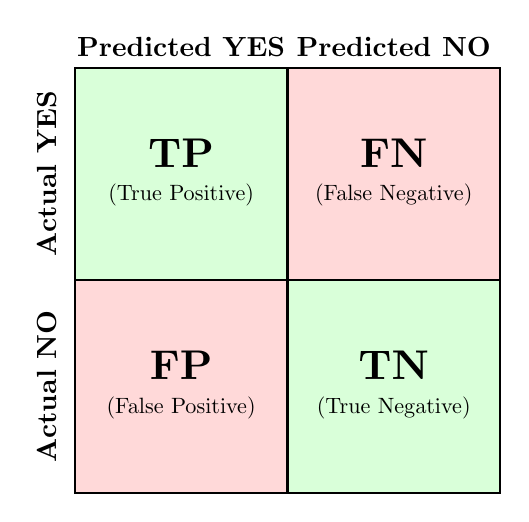
\begin{tikzpicture}[scale=0.9]
        % Labels
        \node[font=\bfseries] at (1.5, 3.3) {Predicted YES};
        \node[font=\bfseries] at (4.5, 3.3) {Predicted NO};
        \node[rotate=90, font=\bfseries] at (-0.4, 1.5) {Actual YES};
        \node[rotate=90, font=\bfseries] at (-0.4, -1.5) {Actual NO};

        % Boxes
        % TP (Green)
        \draw[fill=green!15, thick] (0,0) rectangle (3,3);
        \node[scale=1.5, font=\bfseries] at (1.5, 1.8) {TP};
        \node[scale=0.8] at (1.5, 1.2) {(True Positive)};
        
        % FN (Red)
        \draw[fill=red!15, thick] (3,0) rectangle (6,3);
        \node[scale=1.5, font=\bfseries] at (4.5, 1.8) {FN};
        \node[scale=0.8] at (4.5, 1.2) {(False Negative)};
        
        % FP (Orange)
        \draw[fill=red!15, thick] (0,-3) rectangle (3,0);
        \node[scale=1.5, font=\bfseries] at (1.5, -1.2) {FP};
        \node[scale=0.8] at (1.5, -1.8) {(False Positive)};
        
        % TN (Green)
        \draw[fill=green!15, thick] (3,-3) rectangle (6,0);
        \node[scale=1.5, font=\bfseries] at (4.5, -1.2) {TN};
        \node[scale=0.8] at (4.5, -1.8) {(True Negative)};
    \end{tikzpicture}
\end{frame}

% --- SLIDE 5: PRECISION ---
\begin{frame}{Metric: Precision}
    
    \begin{block}{Question}
        \textit{"Of all the times the model predicted \textbf{YES}, how often was it right?"}
    \end{block}

    \vspace{1em}
    
    \[
        \text{Precision} = \frac{\text{True Positives}}{\text{True Positives} + \textbf{False Positives}}
    \]
    
    \vspace{1.5em}
    
    \textbf{When to use it?}
    \begin{itemize}
        \item When \textbf{False Positives} are expensive/annoying.
        \item \textbf{Example: Spam Filter.} 
        \item We do \textbf{not} want to mark a real email (work, family) as Spam. Better to let a few spam emails through than delete a real one.
    \end{itemize}

\end{frame}

% --- SLIDE 6: RECALL ---
\begin{frame}{Metric: Recall}
    
    \begin{block}{Question}
        \textit{"Of all the \textbf{Real YES} cases in the world, how many did we find?"}
    \end{block}

    \vspace{1em}
    
    \[
        \text{Recall} = \frac{\text{True Positives}}{\text{True Positives} + \textbf{False Negatives}}
    \]
    
    \vspace{1.5em}
    
    \textbf{When to use it?}
    \begin{itemize}
        \item When \textbf{False Negatives} are dangerous/fatal.
        \item \textbf{Example: Cancer/Fraud Detection.} 
        \item We must find \textbf{every} sick patient. It is okay to raise a false alarm (do more tests), but we cannot miss a sick person.
    \end{itemize}

\end{frame}

% --- SLIDE 7: F1 SCORE ---
\begin{frame}{Metric: F1-Score}

    \begin{itemize}
        \item Often we need a balance between Precision and Recall.
        \item If you optimize only one, the other usually suffers (Precision-Recall Tradeoff).
    \end{itemize}

    \vspace{1em}
    
    \begin{block}{F1-Score (Harmonic Mean of Precision and Recall)}
        \[
            F1 = 2 \times \frac{\text{Precision} \times \text{Recall}}{\text{Precision} + \text{Recall}}
        \]
    \end{block}
    
    \begin{itemize}
        \item Used for imbalanced data.
    \end{itemize}
    
    \textbf{Why Harmonic Mean not Arithmetic Mean?}
    \begin{itemize}
        \item It forces the model to be good at \textbf{both}. If Precision is 100\% but Recall is 0\%, the Average is 50\%, but the \textbf{F1-Score is 0}.
    \end{itemize}

\end{frame}

% --- SLIDE 6: BASELINE ---

\begin{frame}{How to know if a specific score is good?}

    \textbf{Question:} My F1-Score is 40\%. Is that good?
\end{frame}
    
\begin{frame}{Baselines}

    \textbf{Question:} My F1-Score is 40\%. Is that good?
    \vspace{0.5em}
    \\
    \textbf{Answer:} Compare it to a "Dummy" Baseline!
    
    \vspace{1em}
    
    \begin{columns}[T]
        \begin{column}{0.48\textwidth}
            \textbf{Classification Baseline}
            \begin{itemize}
                \item Always predict the \textbf{Majority Class}.
                \item If your model can't beat this, it hasn't learned anything.
            \end{itemize}
        \end{column}
        \begin{column}{0.48\textwidth}
            \textbf{Regression Baseline}
            \begin{itemize}
                \item MSE baseline: Use the \textbf{Mean}.
                \item MAE baseline: Use the \textbf{Median}.
                \item If your model can't beat this, you are doing worse than just guessing the average/median!
            \end{itemize}
        \end{column}
    \end{columns}
    
\end{frame}

\subsection{Overfitting Mitigation}
